% Options for packages loaded elsewhere
\PassOptionsToPackage{unicode}{hyperref}
\PassOptionsToPackage{hyphens}{url}
%
\documentclass[
]{article}
\usepackage{lmodern}
\usepackage{amssymb,amsmath}
\usepackage{ifxetex,ifluatex}
\ifnum 0\ifxetex 1\fi\ifluatex 1\fi=0 % if pdftex
  \usepackage[T1]{fontenc}
  \usepackage[utf8]{inputenc}
  \usepackage{textcomp} % provide euro and other symbols
\else % if luatex or xetex
  \usepackage{unicode-math}
  \defaultfontfeatures{Scale=MatchLowercase}
  \defaultfontfeatures[\rmfamily]{Ligatures=TeX,Scale=1}
\fi
% Use upquote if available, for straight quotes in verbatim environments
\IfFileExists{upquote.sty}{\usepackage{upquote}}{}
\IfFileExists{microtype.sty}{% use microtype if available
  \usepackage[]{microtype}
  \UseMicrotypeSet[protrusion]{basicmath} % disable protrusion for tt fonts
}{}
\makeatletter
\@ifundefined{KOMAClassName}{% if non-KOMA class
  \IfFileExists{parskip.sty}{%
    \usepackage{parskip}
  }{% else
    \setlength{\parindent}{0pt}
    \setlength{\parskip}{6pt plus 2pt minus 1pt}}
}{% if KOMA class
  \KOMAoptions{parskip=half}}
\makeatother
\usepackage{xcolor}
\IfFileExists{xurl.sty}{\usepackage{xurl}}{} % add URL line breaks if available
\IfFileExists{bookmark.sty}{\usepackage{bookmark}}{\usepackage{hyperref}}
\hypersetup{
  pdftitle={HarvardX Capstone: MovieLens},
  pdfauthor={Somosree Banerjee},
  hidelinks,
  pdfcreator={LaTeX via pandoc}}
\urlstyle{same} % disable monospaced font for URLs
\usepackage[margin=1in]{geometry}
\usepackage{color}
\usepackage{fancyvrb}
\newcommand{\VerbBar}{|}
\newcommand{\VERB}{\Verb[commandchars=\\\{\}]}
\DefineVerbatimEnvironment{Highlighting}{Verbatim}{commandchars=\\\{\}}
% Add ',fontsize=\small' for more characters per line
\usepackage{framed}
\definecolor{shadecolor}{RGB}{248,248,248}
\newenvironment{Shaded}{\begin{snugshade}}{\end{snugshade}}
\newcommand{\AlertTok}[1]{\textcolor[rgb]{0.94,0.16,0.16}{#1}}
\newcommand{\AnnotationTok}[1]{\textcolor[rgb]{0.56,0.35,0.01}{\textbf{\textit{#1}}}}
\newcommand{\AttributeTok}[1]{\textcolor[rgb]{0.77,0.63,0.00}{#1}}
\newcommand{\BaseNTok}[1]{\textcolor[rgb]{0.00,0.00,0.81}{#1}}
\newcommand{\BuiltInTok}[1]{#1}
\newcommand{\CharTok}[1]{\textcolor[rgb]{0.31,0.60,0.02}{#1}}
\newcommand{\CommentTok}[1]{\textcolor[rgb]{0.56,0.35,0.01}{\textit{#1}}}
\newcommand{\CommentVarTok}[1]{\textcolor[rgb]{0.56,0.35,0.01}{\textbf{\textit{#1}}}}
\newcommand{\ConstantTok}[1]{\textcolor[rgb]{0.00,0.00,0.00}{#1}}
\newcommand{\ControlFlowTok}[1]{\textcolor[rgb]{0.13,0.29,0.53}{\textbf{#1}}}
\newcommand{\DataTypeTok}[1]{\textcolor[rgb]{0.13,0.29,0.53}{#1}}
\newcommand{\DecValTok}[1]{\textcolor[rgb]{0.00,0.00,0.81}{#1}}
\newcommand{\DocumentationTok}[1]{\textcolor[rgb]{0.56,0.35,0.01}{\textbf{\textit{#1}}}}
\newcommand{\ErrorTok}[1]{\textcolor[rgb]{0.64,0.00,0.00}{\textbf{#1}}}
\newcommand{\ExtensionTok}[1]{#1}
\newcommand{\FloatTok}[1]{\textcolor[rgb]{0.00,0.00,0.81}{#1}}
\newcommand{\FunctionTok}[1]{\textcolor[rgb]{0.00,0.00,0.00}{#1}}
\newcommand{\ImportTok}[1]{#1}
\newcommand{\InformationTok}[1]{\textcolor[rgb]{0.56,0.35,0.01}{\textbf{\textit{#1}}}}
\newcommand{\KeywordTok}[1]{\textcolor[rgb]{0.13,0.29,0.53}{\textbf{#1}}}
\newcommand{\NormalTok}[1]{#1}
\newcommand{\OperatorTok}[1]{\textcolor[rgb]{0.81,0.36,0.00}{\textbf{#1}}}
\newcommand{\OtherTok}[1]{\textcolor[rgb]{0.56,0.35,0.01}{#1}}
\newcommand{\PreprocessorTok}[1]{\textcolor[rgb]{0.56,0.35,0.01}{\textit{#1}}}
\newcommand{\RegionMarkerTok}[1]{#1}
\newcommand{\SpecialCharTok}[1]{\textcolor[rgb]{0.00,0.00,0.00}{#1}}
\newcommand{\SpecialStringTok}[1]{\textcolor[rgb]{0.31,0.60,0.02}{#1}}
\newcommand{\StringTok}[1]{\textcolor[rgb]{0.31,0.60,0.02}{#1}}
\newcommand{\VariableTok}[1]{\textcolor[rgb]{0.00,0.00,0.00}{#1}}
\newcommand{\VerbatimStringTok}[1]{\textcolor[rgb]{0.31,0.60,0.02}{#1}}
\newcommand{\WarningTok}[1]{\textcolor[rgb]{0.56,0.35,0.01}{\textbf{\textit{#1}}}}
\usepackage{graphicx,grffile}
\makeatletter
\def\maxwidth{\ifdim\Gin@nat@width>\linewidth\linewidth\else\Gin@nat@width\fi}
\def\maxheight{\ifdim\Gin@nat@height>\textheight\textheight\else\Gin@nat@height\fi}
\makeatother
% Scale images if necessary, so that they will not overflow the page
% margins by default, and it is still possible to overwrite the defaults
% using explicit options in \includegraphics[width, height, ...]{}
\setkeys{Gin}{width=\maxwidth,height=\maxheight,keepaspectratio}
% Set default figure placement to htbp
\makeatletter
\def\fps@figure{htbp}
\makeatother
\setlength{\emergencystretch}{3em} % prevent overfull lines
\providecommand{\tightlist}{%
  \setlength{\itemsep}{0pt}\setlength{\parskip}{0pt}}
\setcounter{secnumdepth}{-\maxdimen} % remove section numbering

\title{HarvardX Capstone: MovieLens}
\author{Somosree Banerjee}
\date{11/03/2020}

\begin{document}
\maketitle

{
\setcounter{tocdepth}{2}
\tableofcontents
}
\hypertarget{i.-introduction}{%
\subsection{I. Introduction}\label{i.-introduction}}

This report is part of the capstone project of the EdX course
``HarvardX: PH125.9x Data Science: Capstone''. The goal is to challenge
and demonstrate how the knowledge acquired through the different topics
covered in ``HarvardX: PH125.9x Data Science'' can be applied in solving
real world problems.

\hypertarget{ii.-summary}{%
\subsection{II. Summary}\label{ii.-summary}}

For the MovieLens project, the data set provided is generated by the
GroupLens research lab. The aim to create a recommendation system using
the ``prediction version of problem''. The report is split in three
sections: 1. Data Loading and Data Wrangling for further Analysis 2.
Data Exploration and Analysis to understand the structure of the data
set. 3. A machine learning algorithm to calculate RMSE. ``Penalized
Least Square Approach'' has been considered to calculate the RMSE.

\hypertarget{iii.-data-loading-and-data-wrangling}{%
\subsection{III. Data Loading and Data
Wrangling}\label{iii.-data-loading-and-data-wrangling}}

\hypertarget{libraries-loaded}{%
\subsection{Libraries Loaded}\label{libraries-loaded}}

library(tidyverse) library(caret) library(data.table)
library(splitstackshape) library(DT) library(lubridate)

The data set `movielens' gets split into a training-test set called
`edx' and a set for validation purposes called `validation'.

\begin{Shaded}
\begin{Highlighting}[]
\CommentTok{################################}
\CommentTok{# Create edx set, validation set}
\CommentTok{################################}
\CommentTok{#Memory }
\KeywordTok{memory.limit}\NormalTok{()}
\end{Highlighting}
\end{Shaded}

\begin{verbatim}
## [1] 8031
\end{verbatim}

\begin{Shaded}
\begin{Highlighting}[]
\KeywordTok{memory.limit}\NormalTok{(}\DataTypeTok{size=}\DecValTok{56000}\NormalTok{)}
\end{Highlighting}
\end{Shaded}

\begin{verbatim}
## [1] 56000
\end{verbatim}

\begin{Shaded}
\begin{Highlighting}[]
\ControlFlowTok{if}\NormalTok{(}\OperatorTok{!}\KeywordTok{require}\NormalTok{(tidyverse)) }\KeywordTok{install.packages}\NormalTok{(}\StringTok{"tidyverse"}\NormalTok{, }\DataTypeTok{repos =} \StringTok{"http://cran.us.r-project.org"}\NormalTok{)}
\end{Highlighting}
\end{Shaded}

\begin{verbatim}
## Loading required package: tidyverse
\end{verbatim}

\begin{verbatim}
## -- Attaching packages ---------------------------- tidyverse 1.3.0 --
\end{verbatim}

\begin{verbatim}
## <U+2713> ggplot2 3.2.1     <U+2713> purrr   0.3.3
## <U+2713> tibble  2.1.3     <U+2713> dplyr   0.8.3
## <U+2713> tidyr   1.0.0     <U+2713> stringr 1.4.0
## <U+2713> readr   1.3.1     <U+2713> forcats 0.4.0
\end{verbatim}

\begin{verbatim}
## -- Conflicts ------------------------------- tidyverse_conflicts() --
## x dplyr::filter() masks stats::filter()
## x dplyr::lag()    masks stats::lag()
\end{verbatim}

\begin{Shaded}
\begin{Highlighting}[]
\ControlFlowTok{if}\NormalTok{(}\OperatorTok{!}\KeywordTok{require}\NormalTok{(caret)) }\KeywordTok{install.packages}\NormalTok{(}\StringTok{"caret"}\NormalTok{, }\DataTypeTok{repos =} \StringTok{"http://cran.us.r-project.org"}\NormalTok{)}
\end{Highlighting}
\end{Shaded}

\begin{verbatim}
## Loading required package: caret
\end{verbatim}

\begin{verbatim}
## Loading required package: lattice
\end{verbatim}

\begin{verbatim}
## 
## Attaching package: 'caret'
\end{verbatim}

\begin{verbatim}
## The following object is masked from 'package:purrr':
## 
##     lift
\end{verbatim}

\begin{Shaded}
\begin{Highlighting}[]
\ControlFlowTok{if}\NormalTok{(}\OperatorTok{!}\KeywordTok{require}\NormalTok{(data.table)) }\KeywordTok{install.packages}\NormalTok{(}\StringTok{"data.table"}\NormalTok{, }\DataTypeTok{repos =} \StringTok{"http://cran.us.r-project.org"}\NormalTok{)}
\end{Highlighting}
\end{Shaded}

\begin{verbatim}
## Loading required package: data.table
\end{verbatim}

\begin{verbatim}
## 
## Attaching package: 'data.table'
\end{verbatim}

\begin{verbatim}
## The following objects are masked from 'package:dplyr':
## 
##     between, first, last
\end{verbatim}

\begin{verbatim}
## The following object is masked from 'package:purrr':
## 
##     transpose
\end{verbatim}

\begin{Shaded}
\begin{Highlighting}[]
\ControlFlowTok{if}\NormalTok{(}\OperatorTok{!}\KeywordTok{require}\NormalTok{(splitstackshape)) }\KeywordTok{install.packages}\NormalTok{(}\StringTok{"splitstackshape"}\NormalTok{, }\DataTypeTok{repos =} \StringTok{"http://cran.us.r-project.org"}\NormalTok{)}
\end{Highlighting}
\end{Shaded}

\begin{verbatim}
## Loading required package: splitstackshape
\end{verbatim}

\begin{verbatim}
## Warning: package 'splitstackshape' was built under R version 3.6.3
\end{verbatim}

\begin{Shaded}
\begin{Highlighting}[]
\ControlFlowTok{if}\NormalTok{(}\OperatorTok{!}\KeywordTok{require}\NormalTok{(DT)) }\KeywordTok{install.packages}\NormalTok{(}\StringTok{"DT"}\NormalTok{, }\DataTypeTok{repos =} \StringTok{"http://cran.us.r-project.org"}\NormalTok{)}
\end{Highlighting}
\end{Shaded}

\begin{verbatim}
## Loading required package: DT
\end{verbatim}

\begin{verbatim}
## Warning: package 'DT' was built under R version 3.6.3
\end{verbatim}

\begin{Shaded}
\begin{Highlighting}[]
\ControlFlowTok{if}\NormalTok{(}\OperatorTok{!}\KeywordTok{require}\NormalTok{(lubridate)) }\KeywordTok{install.packages}\NormalTok{(}\StringTok{"lubridate"}\NormalTok{, }\DataTypeTok{repos =} \StringTok{"http://cran.us.r-project.org"}\NormalTok{)}
\end{Highlighting}
\end{Shaded}

\begin{verbatim}
## Loading required package: lubridate
\end{verbatim}

\begin{verbatim}
## Warning: package 'lubridate' was built under R version 3.6.3
\end{verbatim}

\begin{verbatim}
## 
## Attaching package: 'lubridate'
\end{verbatim}

\begin{verbatim}
## The following objects are masked from 'package:data.table':
## 
##     hour, isoweek, mday, minute, month, quarter, second, wday, week,
##     yday, year
\end{verbatim}

\begin{verbatim}
## The following object is masked from 'package:base':
## 
##     date
\end{verbatim}

\begin{Shaded}
\begin{Highlighting}[]
\KeywordTok{library}\NormalTok{(tidyverse)}
\KeywordTok{library}\NormalTok{(caret)}
\KeywordTok{library}\NormalTok{(data.table)}
\KeywordTok{library}\NormalTok{(splitstackshape)}
\KeywordTok{library}\NormalTok{(DT)}
\KeywordTok{library}\NormalTok{(lubridate)}
\CommentTok{# MovieLens 10M dataset:}
\CommentTok{# https://grouplens.org/datasets/movielens/10m/}
\CommentTok{# http://files.grouplens.org/datasets/movielens/ml-10m.zip}

\NormalTok{dl <-}\StringTok{ }\KeywordTok{tempfile}\NormalTok{()}
\KeywordTok{download.file}\NormalTok{(}\StringTok{"http://files.grouplens.org/datasets/movielens/ml-10m.zip"}\NormalTok{, dl)}

\NormalTok{ratings <-}\StringTok{ }\KeywordTok{fread}\NormalTok{(}\DataTypeTok{text =} \KeywordTok{gsub}\NormalTok{(}\StringTok{"::"}\NormalTok{, }\StringTok{"}\CharTok{\textbackslash{}t}\StringTok{"}\NormalTok{, }\KeywordTok{readLines}\NormalTok{(}\KeywordTok{unzip}\NormalTok{(dl, }\StringTok{"ml-10M100K/ratings.dat"}\NormalTok{))),}
                 \DataTypeTok{col.names =} \KeywordTok{c}\NormalTok{(}\StringTok{"userId"}\NormalTok{, }\StringTok{"movieId"}\NormalTok{, }\StringTok{"rating"}\NormalTok{, }\StringTok{"timestamp"}\NormalTok{))}
\NormalTok{movies <-}\StringTok{ }\KeywordTok{str_split_fixed}\NormalTok{(}\KeywordTok{readLines}\NormalTok{(}\KeywordTok{unzip}\NormalTok{(dl, }\StringTok{"ml-10M100K/movies.dat"}\NormalTok{)), }\StringTok{"}\CharTok{\textbackslash{}\textbackslash{}}\StringTok{::"}\NormalTok{, }\DecValTok{3}\NormalTok{)}

\KeywordTok{colnames}\NormalTok{(movies) <-}\StringTok{ }\KeywordTok{c}\NormalTok{(}\StringTok{"movieId"}\NormalTok{, }\StringTok{"title"}\NormalTok{, }\StringTok{"genres"}\NormalTok{)}
\NormalTok{movies <-}\StringTok{ }\KeywordTok{as.data.frame}\NormalTok{(movies) }\OperatorTok\StringTok{ }\KeywordTok{mutate}\NormalTok{(}\DataTypeTok{movieId =} \KeywordTok{as.numeric}\NormalTok{(}\KeywordTok{levels}\NormalTok{(movieId))[movieId],}\DataTypeTok{title =} \KeywordTok{as.character}\NormalTok{(title),}
\DataTypeTok{genres =} \KeywordTok{as.character}\NormalTok{(genres))}

\NormalTok{movielens <-}\StringTok{ }\KeywordTok{left_join}\NormalTok{(ratings, movies, }\DataTypeTok{by =} \StringTok{"movieId"}\NormalTok{)}

\CommentTok{# Validation set will be 10% of MovieLens data}
\KeywordTok{set.seed}\NormalTok{(}\DecValTok{1}\NormalTok{, }\DataTypeTok{sample.kind=}\StringTok{"Rounding"}\NormalTok{)}
\end{Highlighting}
\end{Shaded}

\begin{verbatim}
## Warning in set.seed(1, sample.kind = "Rounding"): non-uniform 'Rounding' sampler
## used
\end{verbatim}

\begin{Shaded}
\begin{Highlighting}[]
\CommentTok{# if using R 3.5 or earlier, use `set.seed(1)` instead}
\NormalTok{test_index <-}\StringTok{ }\KeywordTok{createDataPartition}\NormalTok{(}\DataTypeTok{y =}\NormalTok{ movielens}\OperatorTok{$}\NormalTok{rating, }\DataTypeTok{times =} \DecValTok{1}\NormalTok{, }\DataTypeTok{p =} \FloatTok{0.1}\NormalTok{, }\DataTypeTok{list =} \OtherTok{FALSE}\NormalTok{)}
\NormalTok{edx <-}\StringTok{ }\NormalTok{movielens[}\OperatorTok{-}\NormalTok{test_index,]}
\NormalTok{temp <-}\StringTok{ }\NormalTok{movielens[test_index,]}

\CommentTok{# Make sure userId and movieId in validation set are also in edx set}
\NormalTok{validation <-}\StringTok{ }\NormalTok{temp }\OperatorTok\StringTok{ }
\StringTok{  }\KeywordTok{semi_join}\NormalTok{(edx, }\DataTypeTok{by =} \StringTok{"movieId"}\NormalTok{) }\OperatorTok
\StringTok{  }\KeywordTok{semi_join}\NormalTok{(edx, }\DataTypeTok{by =} \StringTok{"userId"}\NormalTok{)}

\CommentTok{# Add rows removed from validation set back into edx set}
\NormalTok{removed <-}\StringTok{ }\KeywordTok{anti_join}\NormalTok{(temp, validation)}
\end{Highlighting}
\end{Shaded}

\begin{verbatim}
## Joining, by = c("userId", "movieId", "rating", "timestamp", "title", "genres")
\end{verbatim}

\begin{Shaded}
\begin{Highlighting}[]
\NormalTok{edx <-}\StringTok{ }\KeywordTok{rbind}\NormalTok{(edx, removed)}

\KeywordTok{rm}\NormalTok{(dl, ratings, movies, test_index, temp, movielens, removed)}
\end{Highlighting}
\end{Shaded}

\hypertarget{iii.-data-exploration-analysis}{%
\subsection{III. Data Exploration \&
Analysis}\label{iii.-data-exploration-analysis}}

\begin{Shaded}
\begin{Highlighting}[]
\KeywordTok{summary}\NormalTok{(edx)}
\end{Highlighting}
\end{Shaded}

\begin{verbatim}
##      userId         movieId          rating        timestamp        
##  Min.   :    1   Min.   :    1   Min.   :0.500   Min.   :7.897e+08  
##  1st Qu.:18124   1st Qu.:  648   1st Qu.:3.000   1st Qu.:9.468e+08  
##  Median :35738   Median : 1834   Median :4.000   Median :1.035e+09  
##  Mean   :35870   Mean   : 4122   Mean   :3.512   Mean   :1.033e+09  
##  3rd Qu.:53607   3rd Qu.: 3626   3rd Qu.:4.000   3rd Qu.:1.127e+09  
##  Max.   :71567   Max.   :65133   Max.   :5.000   Max.   :1.231e+09  
##     title              genres         
##  Length:9000055     Length:9000055    
##  Class :character   Class :character  
##  Mode  :character   Mode  :character  
##                                       
##                                       
## 
\end{verbatim}

\#Quantitative:Rating Analysis

\hypertarget{table-showing-the-rating-count}{%
\section{Table Showing the Rating
Count}\label{table-showing-the-rating-count}}

\begin{Shaded}
\begin{Highlighting}[]
\KeywordTok{head}\NormalTok{(}\KeywordTok{sort}\NormalTok{(}\KeywordTok{table}\NormalTok{(edx}\OperatorTok{$}\NormalTok{rating)),}\DecValTok{10}\NormalTok{)}
\end{Highlighting}
\end{Shaded}

\begin{verbatim}
## 
##     0.5     1.5     2.5       1     4.5       2     3.5       5       3       4 
##   85374  106426  333010  345679  526736  711422  791624 1390114 2121240 2588430
\end{verbatim}

\#Plot Histogram (Graphical Representation)

\begin{Shaded}
\begin{Highlighting}[]
\KeywordTok{ggplot}\NormalTok{(edx, }\KeywordTok{aes}\NormalTok{(}\DataTypeTok{x=}\NormalTok{ edx}\OperatorTok{$}\NormalTok{rating)) }\OperatorTok{+}
\StringTok{  }\KeywordTok{geom_histogram}\NormalTok{( }\DataTypeTok{binwidth =} \FloatTok{0.2}\NormalTok{) }\OperatorTok{+}
\StringTok{  }\KeywordTok{scale_x_continuous}\NormalTok{(}\DataTypeTok{breaks=}\KeywordTok{seq}\NormalTok{(}\DecValTok{0}\NormalTok{, }\DecValTok{5}\NormalTok{, }\DataTypeTok{by=} \FloatTok{0.5}\NormalTok{)) }\OperatorTok{+}
\StringTok{    }\KeywordTok{labs}\NormalTok{(}\DataTypeTok{x=}\StringTok{"Rating"}\NormalTok{, }\DataTypeTok{y=}\StringTok{"No. of ratings"}\NormalTok{, }\DataTypeTok{caption =} \StringTok{"Source Data: edx set"}\NormalTok{) }\OperatorTok{+}
\StringTok{  }\KeywordTok{ggtitle}\NormalTok{(}\StringTok{"Histogram : Ratings Tally"}\NormalTok{)}
\end{Highlighting}
\end{Shaded}

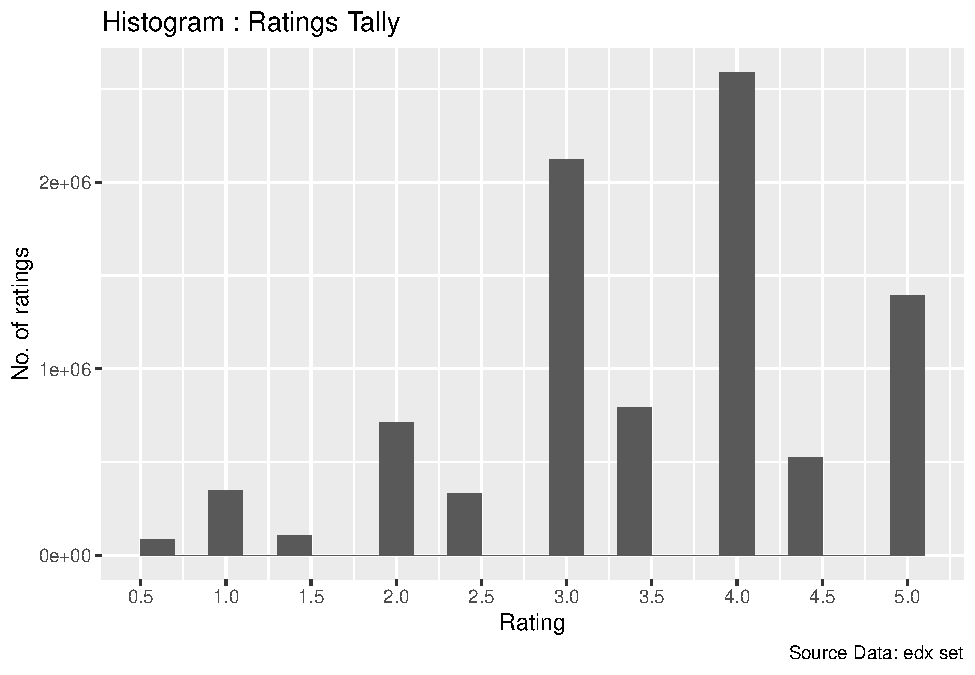
\includegraphics{MovieLensProjectReport_files/figure-latex/ratings Graphical Representation-1.pdf}
\#Conclusions: The above graphical representation concludes the
following facts: 1. No user had given 0 as rating 2. The top 5 ratings
from most to least are : 4, 3, 5, 3.5 and 3. The half star ratings are
less common than whole star ratings.

\#Quantitative:Movie Id Vs Ratings Analysis \#Plot Histogram (Graphical
Representation)

\begin{Shaded}
\begin{Highlighting}[]
\NormalTok{edx }\OperatorTok\StringTok{ }\KeywordTok{group_by}\NormalTok{(movieId) }\OperatorTok\StringTok{ }\KeywordTok{summarize}\NormalTok{(}\DataTypeTok{n =} \KeywordTok{n}\NormalTok{()) }\OperatorTok
\StringTok{  }\KeywordTok{ggplot}\NormalTok{(}\KeywordTok{aes}\NormalTok{(movieId)) }\OperatorTok{+}\StringTok{ }\KeywordTok{geom_histogram}\NormalTok{(}\DataTypeTok{bins =} \DecValTok{10}\NormalTok{) }\OperatorTok{+}
\StringTok{  }\KeywordTok{labs}\NormalTok{(}\DataTypeTok{x=}\StringTok{"MovieID"}\NormalTok{, }\DataTypeTok{y=}\StringTok{"No. of ratings"}\NormalTok{, }\DataTypeTok{caption =} \StringTok{"Source Data: edx set"}\NormalTok{) }\OperatorTok{+}
\StringTok{  }\KeywordTok{ggtitle}\NormalTok{(}\StringTok{"Number of Movies Ratings"}\NormalTok{)}
\end{Highlighting}
\end{Shaded}

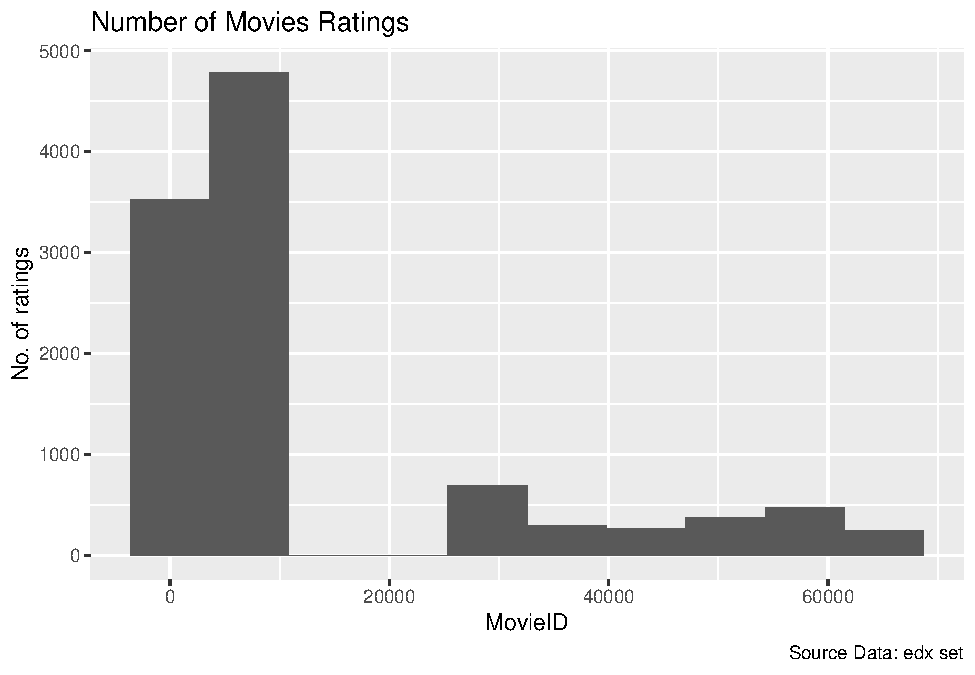
\includegraphics{MovieLensProjectReport_files/figure-latex/MovieId-1.pdf}
\#Conclusion: The above graphical representation for MovieID depicts
that movies with few ratings tend to have more volatile ratings than
movies which are rated more. \#Quantitative:UserId Vs Ratings Analysis
\#Plot Histogram (Graphical Representation)

\begin{Shaded}
\begin{Highlighting}[]
\NormalTok{edx }\OperatorTok\StringTok{ }\KeywordTok{group_by}\NormalTok{(userId) }\OperatorTok\StringTok{ }\KeywordTok{summarize}\NormalTok{(}\DataTypeTok{n =} \KeywordTok{n}\NormalTok{()) }\OperatorTok
\StringTok{  }\KeywordTok{ggplot}\NormalTok{(}\KeywordTok{aes}\NormalTok{(userId)) }\OperatorTok{+}\StringTok{ }\KeywordTok{geom_histogram}\NormalTok{(}\DataTypeTok{bins =} \DecValTok{10}\NormalTok{) }\OperatorTok{+}
\StringTok{  }\KeywordTok{labs}\NormalTok{(}\DataTypeTok{x=}\StringTok{"UserID"}\NormalTok{, }\DataTypeTok{y=}\StringTok{"No. of ratings"}\NormalTok{, }\DataTypeTok{caption =} \StringTok{"Source Data: edx set"}\NormalTok{) }\OperatorTok{+}
\StringTok{  }\KeywordTok{ggtitle}\NormalTok{(}\StringTok{"Number of User Ratings"}\NormalTok{)}
\end{Highlighting}
\end{Shaded}

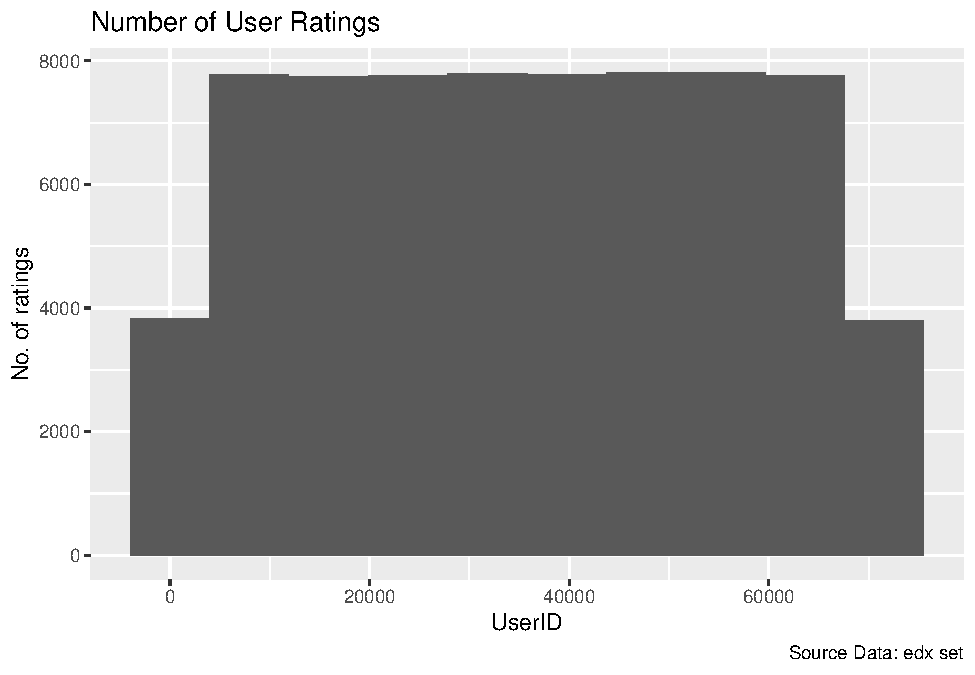
\includegraphics{MovieLensProjectReport_files/figure-latex/UserID-1.pdf}
\#Conclusion: The above graphical representation for User ID depicts
that users who rate just a few movies tend to have more volatile ratings
than users who rate lots of movies \#Qualitative:Genres vs Ratings
Analysis 1. Segregate and extract the Genres from the combination of
Genres

\begin{Shaded}
\begin{Highlighting}[]
\NormalTok{edx_Splitted <-}\StringTok{ }\KeywordTok{cSplit}\NormalTok{(edx, }\StringTok{"genres"}\NormalTok{, }\DataTypeTok{sep =} \StringTok{"|"}\NormalTok{ ,  }\DataTypeTok{direction =} \StringTok{"long"}\NormalTok{)}
\end{Highlighting}
\end{Shaded}

\begin{enumerate}
\def\labelenumi{\arabic{enumi}.}
\setcounter{enumi}{1}
\tightlist
\item
  Calculate the Rating Count per Genre
\end{enumerate}

\begin{Shaded}
\begin{Highlighting}[]
\NormalTok{edx_Genre_rating <-}\StringTok{ }\NormalTok{edx_Splitted }\OperatorTok\StringTok{ }
\StringTok{  }\KeywordTok{group_by}\NormalTok{(genres) }\OperatorTok
\StringTok{  }\KeywordTok{summarize}\NormalTok{(}\DataTypeTok{RatingCount =} \KeywordTok{n}\NormalTok{()) }\OperatorTok
\StringTok{  }\KeywordTok{arrange}\NormalTok{(}\KeywordTok{desc}\NormalTok{(RatingCount))}
\CommentTok{#Tabular Representation}
\KeywordTok{datatable}\NormalTok{(edx_Genre_rating, }\DataTypeTok{rownames =} \OtherTok{FALSE}\NormalTok{, }\DataTypeTok{filter=}\StringTok{"top"}\NormalTok{, }\DataTypeTok{options =} \KeywordTok{list}\NormalTok{(}\DataTypeTok{pageLength =} \DecValTok{50}\NormalTok{, }\DataTypeTok{scrollX=}\NormalTok{T) ) }\OperatorTok
\StringTok{  }\KeywordTok{formatRound}\NormalTok{(}\StringTok{'RatingCount'}\NormalTok{,}\DataTypeTok{digits=}\DecValTok{0}\NormalTok{, }\DataTypeTok{interval =} \DecValTok{3}\NormalTok{, }\DataTypeTok{mark =} \StringTok{","}\NormalTok{)}
\end{Highlighting}
\end{Shaded}

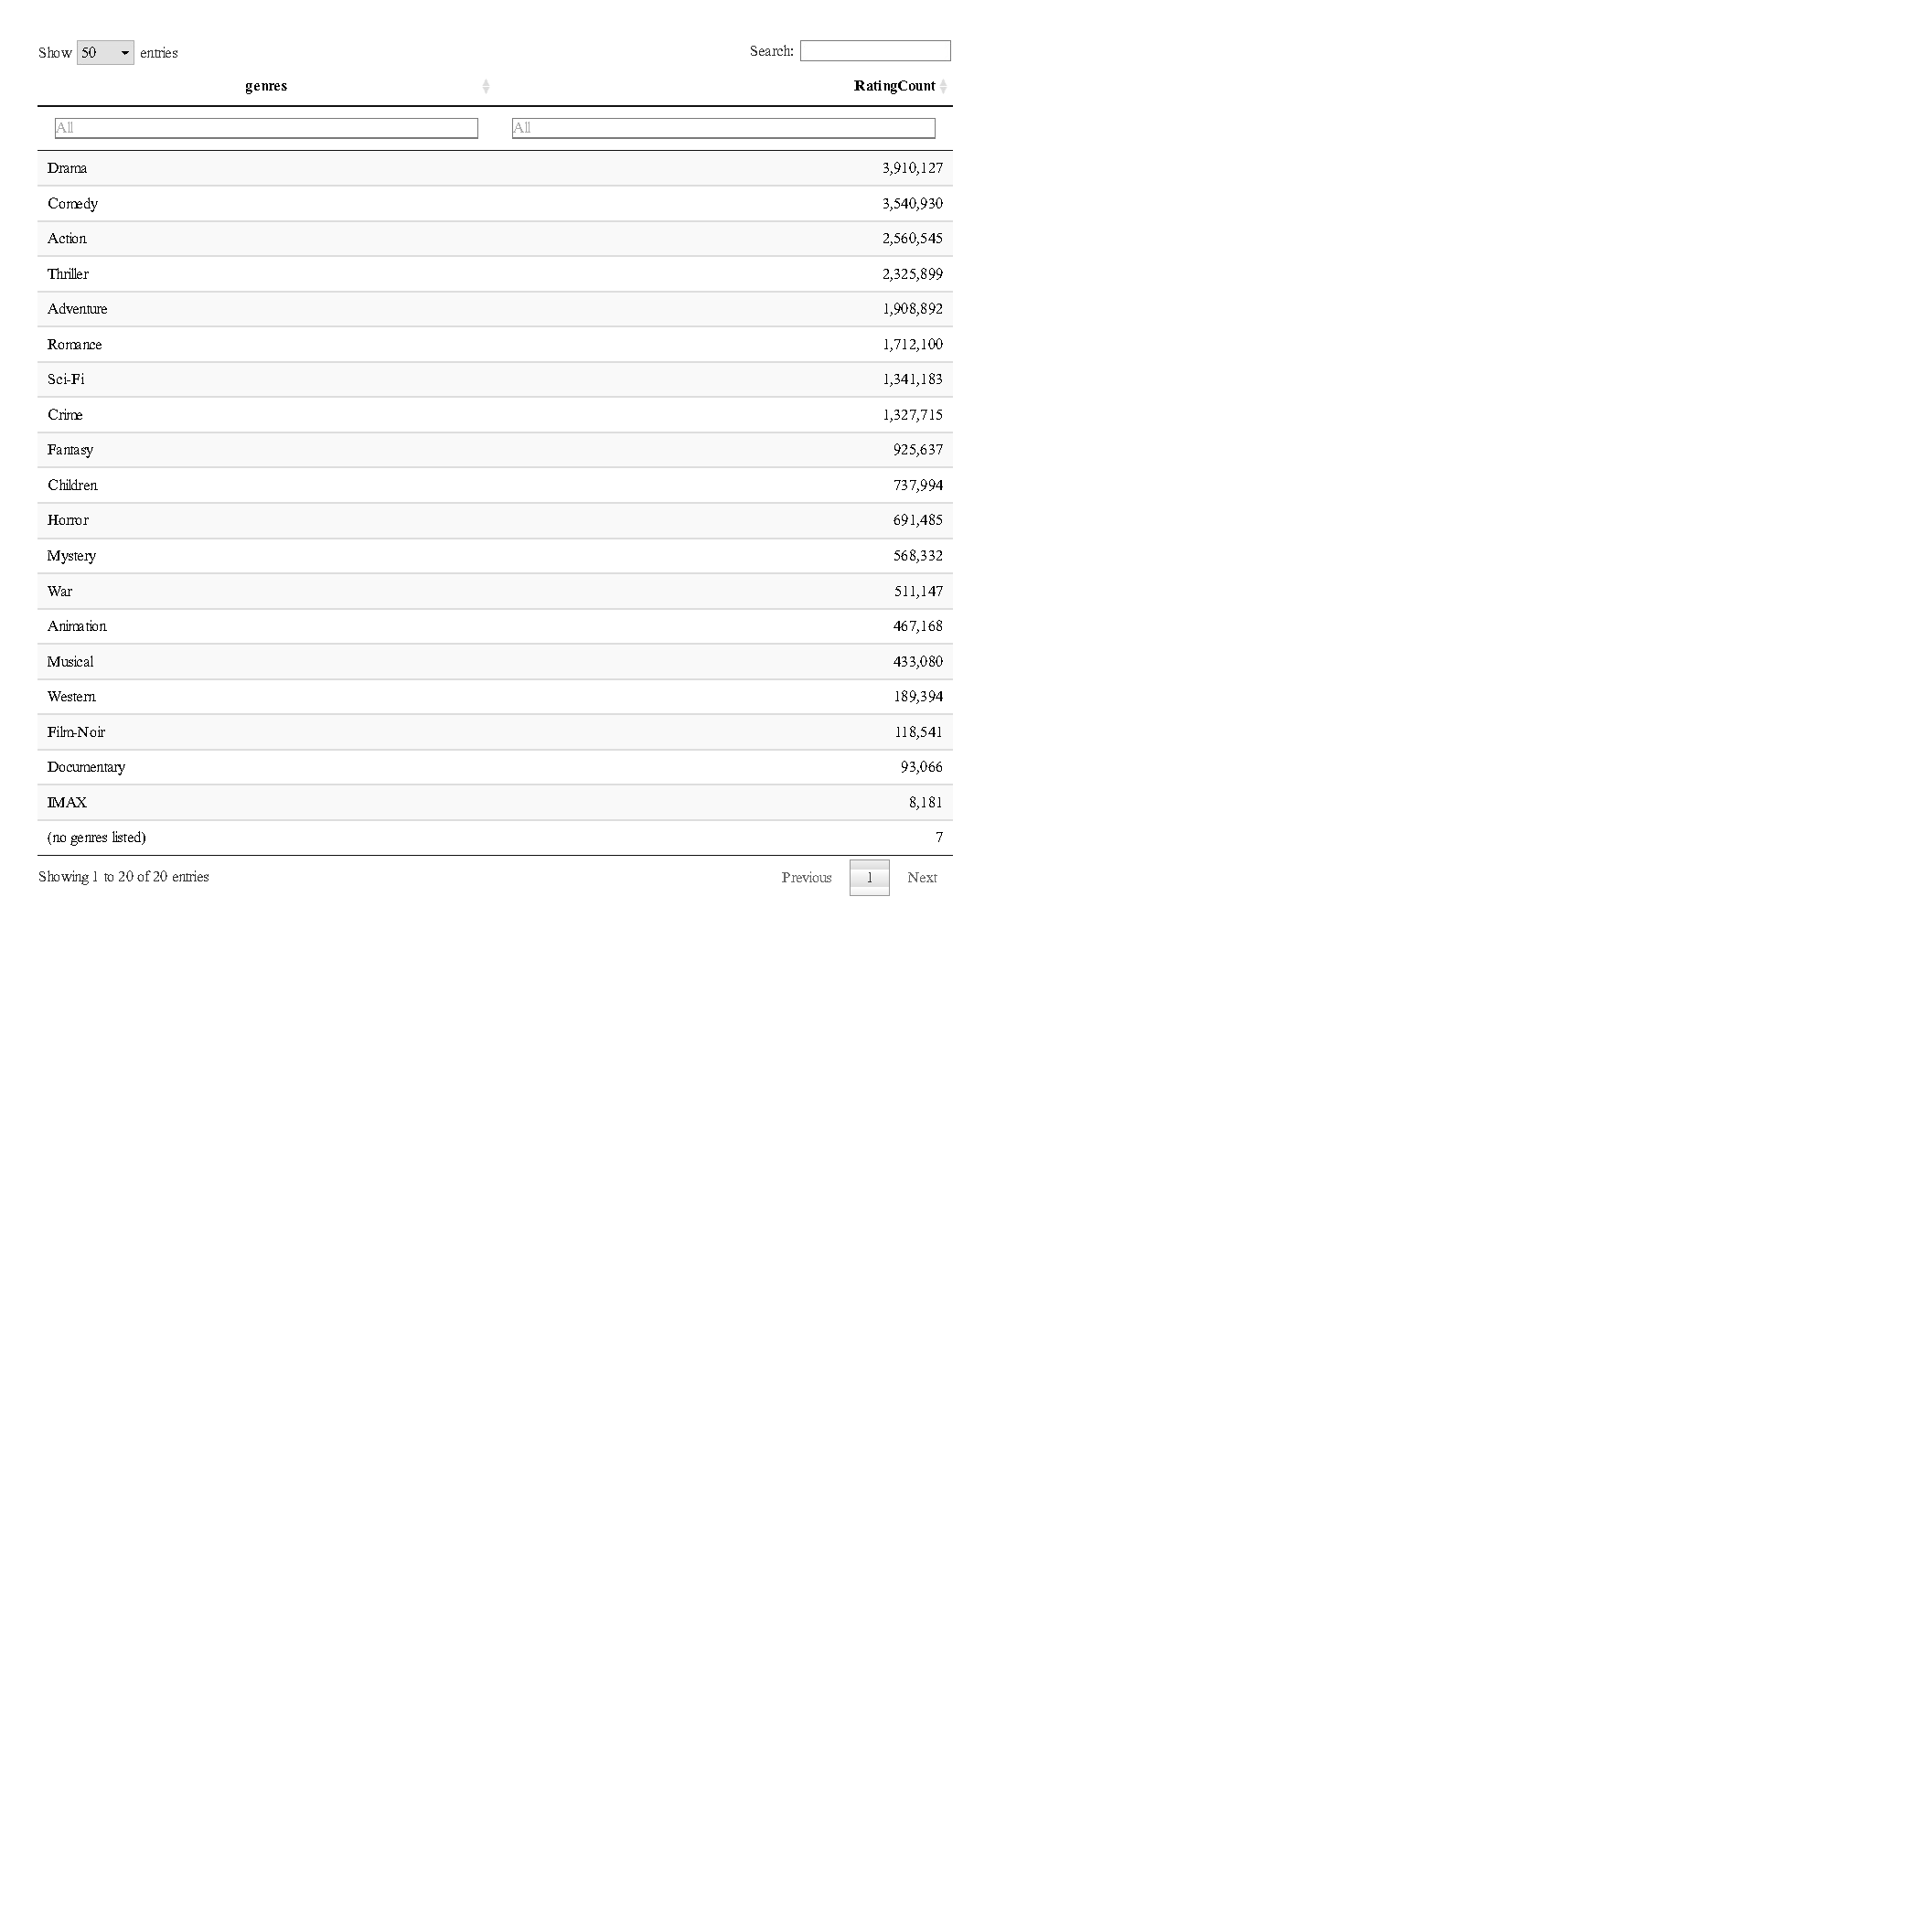
\includegraphics{MovieLensProjectReport_files/figure-latex/genres Rating Count-1.pdf}
\#Graphical representation (Point Chart)

\begin{Shaded}
\begin{Highlighting}[]
\KeywordTok{ggplot}\NormalTok{(edx_Genre_rating, }\KeywordTok{aes}\NormalTok{(}\DataTypeTok{x=}\NormalTok{ genres, }\DataTypeTok{y=}\NormalTok{RatingCount)) }\OperatorTok{+}
\StringTok{  }\KeywordTok{geom_point}\NormalTok{() }\OperatorTok{+}
\StringTok{  }\KeywordTok{theme}\NormalTok{(}\DataTypeTok{axis.text.x =} \KeywordTok{element_text}\NormalTok{(}\DataTypeTok{angle =} \DecValTok{90}\NormalTok{,}\DataTypeTok{hjust =} \DecValTok{1}\NormalTok{))}\OperatorTok{+}
\StringTok{  }\KeywordTok{scale_y_continuous}\NormalTok{(}\DataTypeTok{trans =} \StringTok{"log2"}\NormalTok{)}\OperatorTok{+}
\StringTok{  }\KeywordTok{ggtitle}\NormalTok{(}\StringTok{"Genre - Ratings Point Chart"}\NormalTok{)}
\end{Highlighting}
\end{Shaded}

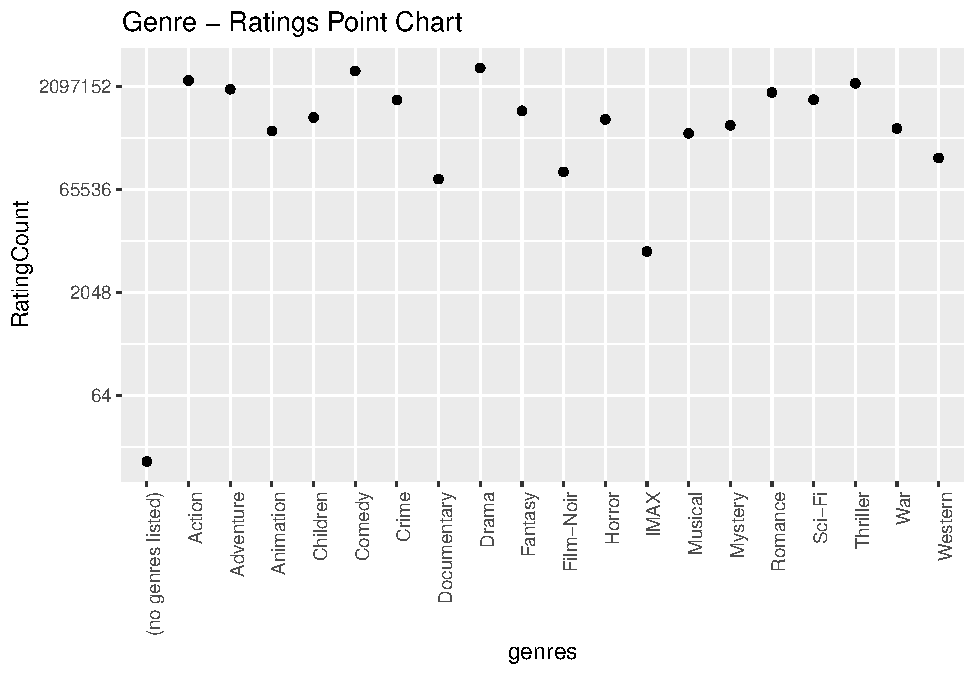
\includegraphics{MovieLensProjectReport_files/figure-latex/genres Graphical Plot-1.pdf}
\#Conclusion: The above tabular and graphical representation concludes
that three Genres with the highest Rating count are: 1. Drama 2. Comedy
3. Action Movies with ``no genre'' have least movie ratings (7).

\#Qualitative:Movie Titles vs Ratings Analysis Calculate the Rating
Count per Movie

\begin{Shaded}
\begin{Highlighting}[]
\NormalTok{edx_Movie_Ratings <-}\StringTok{ }\NormalTok{edx }\OperatorTok\StringTok{ }
\StringTok{  }\KeywordTok{group_by}\NormalTok{(title, genres) }\OperatorTok
\StringTok{  }\KeywordTok{summarize}\NormalTok{(}\DataTypeTok{RatingCount =} \KeywordTok{n}\NormalTok{()) }\OperatorTok
\StringTok{  }\KeywordTok{arrange}\NormalTok{(}\KeywordTok{desc}\NormalTok{(RatingCount))}
\CommentTok{#Tabular Representation}
\KeywordTok{datatable}\NormalTok{(edx_Movie_Ratings, }\DataTypeTok{rownames =} \OtherTok{FALSE}\NormalTok{, }\DataTypeTok{filter=}\StringTok{"top"}\NormalTok{, }\DataTypeTok{options =} \KeywordTok{list}\NormalTok{(}\DataTypeTok{pageLength =} \DecValTok{10}\NormalTok{, }\DataTypeTok{scrollX=}\NormalTok{T) ) }\OperatorTok
\StringTok{  }\KeywordTok{formatRound}\NormalTok{(}\StringTok{'RatingCount'}\NormalTok{,}\DataTypeTok{digits=}\DecValTok{0}\NormalTok{, }\DataTypeTok{interval =} \DecValTok{3}\NormalTok{, }\DataTypeTok{mark =} \StringTok{","}\NormalTok{)}
\end{Highlighting}
\end{Shaded}

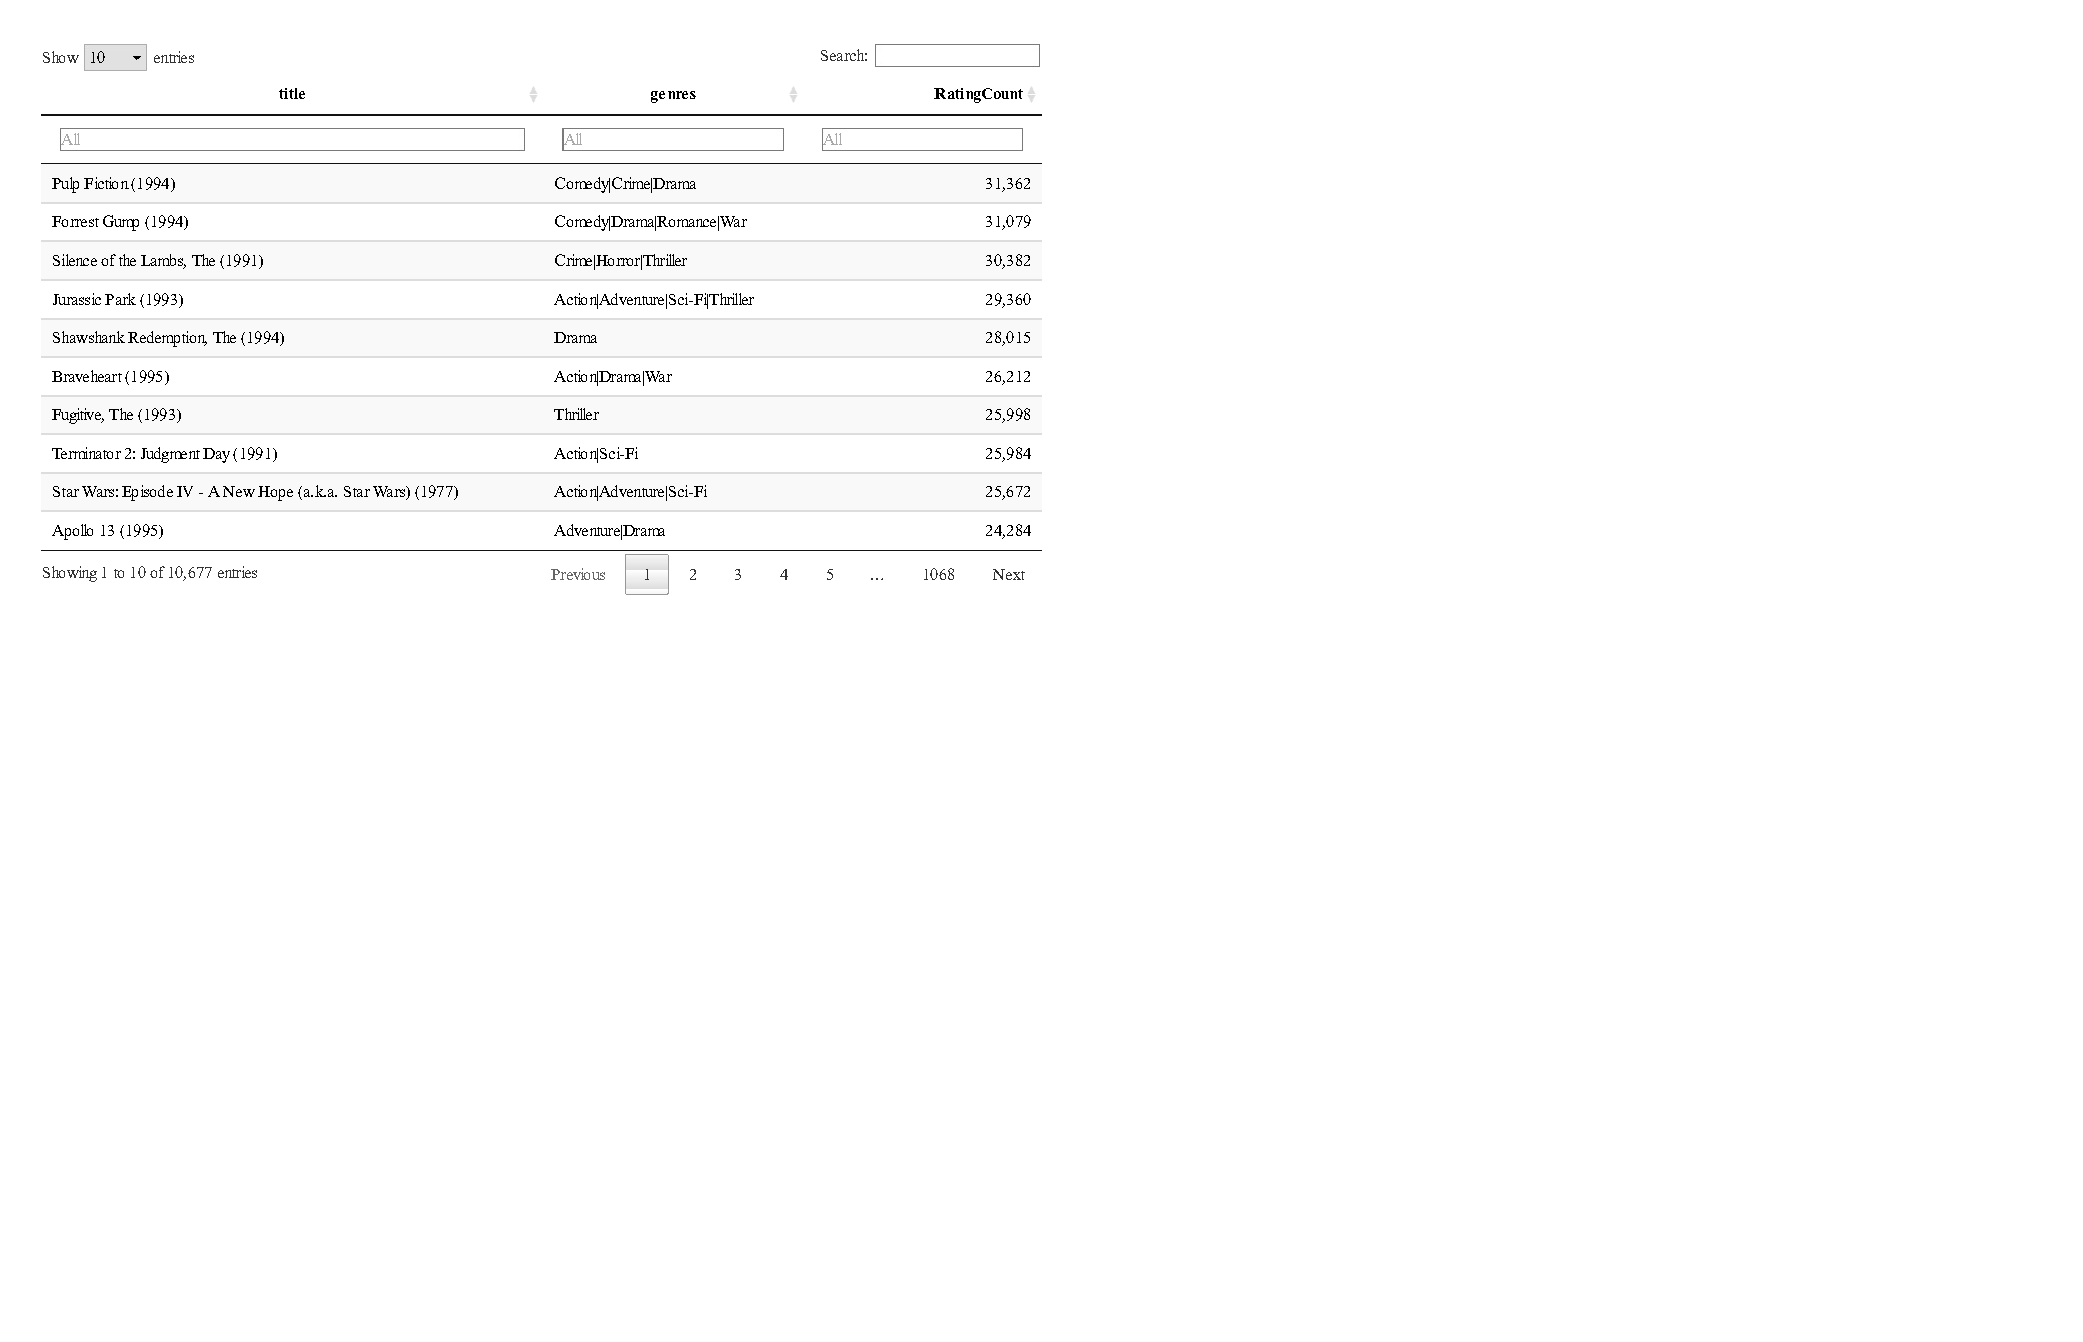
\includegraphics{MovieLensProjectReport_files/figure-latex/MovieTitle Tabular Representation-1.pdf}
\#Graphical representation (Bar Chart)

\begin{Shaded}
\begin{Highlighting}[]
\NormalTok{edx }\OperatorTok\StringTok{ }\KeywordTok{group_by}\NormalTok{(title) }\OperatorTok\StringTok{ }\KeywordTok{summarise}\NormalTok{(}\DataTypeTok{count =} \KeywordTok{n}\NormalTok{()) }\OperatorTok\StringTok{ }\KeywordTok{top_n}\NormalTok{(}\DecValTok{10}\NormalTok{,count) }\OperatorTok
\StringTok{  }\KeywordTok{arrange}\NormalTok{(}\KeywordTok{desc}\NormalTok{(count)) }\OperatorTok
\StringTok{  }\KeywordTok{ggplot}\NormalTok{(}\KeywordTok{aes}\NormalTok{(}\DataTypeTok{x=}\KeywordTok{reorder}\NormalTok{(title, count), }\DataTypeTok{y=}\NormalTok{count)) }\OperatorTok{+}\StringTok{ }\KeywordTok{coord_flip}\NormalTok{(}\DataTypeTok{y=}\KeywordTok{c}\NormalTok{(}\DecValTok{0}\NormalTok{, }\DecValTok{40000}\NormalTok{)) }\OperatorTok{+}
\StringTok{  }\KeywordTok{geom_bar}\NormalTok{(}\DataTypeTok{stat=}\StringTok{'identity'}\NormalTok{, }\DataTypeTok{fill=}\StringTok{"purple"}\NormalTok{) }\OperatorTok{+}\StringTok{ }
\StringTok{  }\KeywordTok{labs}\NormalTok{(}\DataTypeTok{x=}\StringTok{""}\NormalTok{, }\DataTypeTok{y=}\StringTok{"Number of ratings"}\NormalTok{) }\OperatorTok{+}
\StringTok{  }\KeywordTok{geom_text}\NormalTok{(}\KeywordTok{aes}\NormalTok{(}\DataTypeTok{label=}\NormalTok{ count), }\DataTypeTok{hjust=}\OperatorTok{-}\FloatTok{0.1}\NormalTok{, }\DataTypeTok{size=}\DecValTok{3}\NormalTok{) }\OperatorTok{+}
\StringTok{  }\KeywordTok{labs}\NormalTok{(}\DataTypeTok{title=}\StringTok{" Top 10 Movies }\CharTok{\textbackslash{}n}\StringTok{ on number on ratings"}\NormalTok{ , }\DataTypeTok{caption =} \StringTok{"source data: edx set"}\NormalTok{)}
\end{Highlighting}
\end{Shaded}

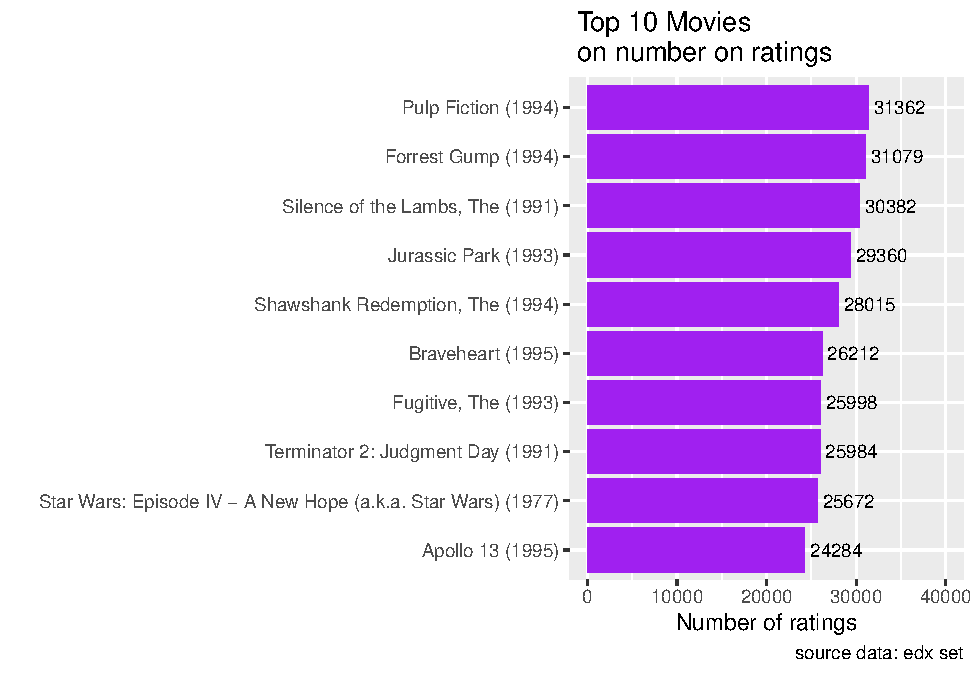
\includegraphics{MovieLensProjectReport_files/figure-latex/MovieTitle Graphical Representation-1.pdf}
\#Conclusion: The above tabular and graphical representation of ``Movie
Title'' confirms previous analysis. The movies which have the highest
number of ratings are in the top genres categories : movies like Pulp
fiction (1994), Forrest Ump(1994) or Jurrasic Park(1993) which are in
the top 5 of movie's ratings number , are part of the Drama, Comedy or
Action genres.

\#Movie Age vs Movie Ratings Extract Premier year from Movie Title

\begin{Shaded}
\begin{Highlighting}[]
\CommentTok{#RegEx could have been used as well, but there are movie titles with number in it resulting in wrong determination of Movie Year}
\NormalTok{PremierYear <-}\StringTok{ }\KeywordTok{as.numeric}\NormalTok{(}\KeywordTok{substr}\NormalTok{(}\KeywordTok{as.character}\NormalTok{(edx}\OperatorTok{$}\NormalTok{title),}\KeywordTok{nchar}\NormalTok{(}\KeywordTok{as.character}\NormalTok{(edx}\OperatorTok{$}\NormalTok{title))}\OperatorTok{-}\DecValTok{4}\NormalTok{,}\KeywordTok{nchar}\NormalTok{(}\KeywordTok{as.character}\NormalTok{(edx}\OperatorTok{$}\NormalTok{title))}\OperatorTok{-}\DecValTok{1}\NormalTok{))}
\end{Highlighting}
\end{Shaded}

Modify the Data Frame with Premier Year and also validate the Premier
Year

\begin{Shaded}
\begin{Highlighting}[]
\NormalTok{edx_Movie_Aging_Details <-}\StringTok{ }\NormalTok{edx }\OperatorTok\StringTok{ }\KeywordTok{mutate}\NormalTok{(}\DataTypeTok{Rated_Year =} \KeywordTok{year}\NormalTok{(}\KeywordTok{as_datetime}\NormalTok{(timestamp)), }\DataTypeTok{Premier_Year =}\NormalTok{ PremierYear) }\OperatorTok\StringTok{ }\KeywordTok{select}\NormalTok{(}\OperatorTok{-}\NormalTok{timestamp)}
\KeywordTok{head}\NormalTok{(edx_Movie_Aging_Details)}
\end{Highlighting}
\end{Shaded}

\begin{verbatim}
##   userId movieId rating                         title
## 1      1     122      5              Boomerang (1992)
## 2      1     185      5               Net, The (1995)
## 3      1     292      5               Outbreak (1995)
## 4      1     316      5               Stargate (1994)
## 5      1     329      5 Star Trek: Generations (1994)
## 6      1     355      5       Flintstones, The (1994)
##                          genres Rated_Year Premier_Year
## 1                Comedy|Romance       1996         1992
## 2         Action|Crime|Thriller       1996         1995
## 3  Action|Drama|Sci-Fi|Thriller       1996         1995
## 4       Action|Adventure|Sci-Fi       1996         1994
## 5 Action|Adventure|Drama|Sci-Fi       1996         1994
## 6       Children|Comedy|Fantasy       1996         1994
\end{verbatim}

\begin{Shaded}
\begin{Highlighting}[]
\NormalTok{edx_Movie_Aging_Details }\OperatorTok\StringTok{ }\KeywordTok{filter}\NormalTok{(Premier_Year }\OperatorTok{<}\StringTok{ }\DecValTok{1900} \OperatorTok{||}\StringTok{ }\NormalTok{Premier_Year }\OperatorTok{>}\StringTok{ }\DecValTok{2018}\NormalTok{) }\OperatorTok\StringTok{ }\KeywordTok{group_by}\NormalTok{(movieId, title, Premier_Year,Rated_Year) }\OperatorTok\StringTok{ }\KeywordTok{summarize}\NormalTok{(}\DataTypeTok{n =} \KeywordTok{n}\NormalTok{())}
\end{Highlighting}
\end{Shaded}

\begin{verbatim}
## # A tibble: 0 x 5
## # Groups:   movieId, title, Premier_Year [0]
## # … with 5 variables: movieId <dbl>, title <chr>, Premier_Year <dbl>,
## #   Rated_Year <dbl>, n <int>
\end{verbatim}

\hypertarget{calculate-movie-age-and-average-rating}{%
\section{Calculate Movie Age and Average
Rating}\label{calculate-movie-age-and-average-rating}}

\begin{Shaded}
\begin{Highlighting}[]
\NormalTok{edx_Movie_Aging_Details_Avg <-}\StringTok{ }\NormalTok{edx_Movie_Aging_Details }\OperatorTok\StringTok{ }
\StringTok{  }\KeywordTok{mutate}\NormalTok{(}\DataTypeTok{Movie_age =} \DecValTok{2018} \OperatorTok{-}\StringTok{ }\NormalTok{Premier_Year) }\OperatorTok\StringTok{ }\KeywordTok{group_by}\NormalTok{(Movie_age) }\OperatorTok\StringTok{ }\KeywordTok{summarize}\NormalTok{(}\DataTypeTok{avg_rating_by_age =} \KeywordTok{mean}\NormalTok{(rating))}\OperatorTok\StringTok{ }\KeywordTok{arrange}\NormalTok{(}\KeywordTok{desc}\NormalTok{(Movie_age))}
\KeywordTok{head}\NormalTok{(edx_Movie_Aging_Details_Avg)}
\end{Highlighting}
\end{Shaded}

\begin{verbatim}
## # A tibble: 6 x 2
##   Movie_age avg_rating_by_age
##       <dbl>             <dbl>
## 1       103              3.29
## 2       102              3.83
## 3       101              3.73
## 4       100              3.65
## 5        99              3.28
## 6        98              3.94
\end{verbatim}

\#Graphical Representation (Point Chart) : Age of movie vs average movie
rating

\begin{Shaded}
\begin{Highlighting}[]
\NormalTok{edx_Movie_Aging_Details_Avg }\OperatorTok
\StringTok{  }\KeywordTok{ggplot}\NormalTok{(}\KeywordTok{aes}\NormalTok{(Movie_age, avg_rating_by_age)) }\OperatorTok{+}
\StringTok{  }\KeywordTok{geom_point}\NormalTok{() }\OperatorTok{+}
\StringTok{  }\KeywordTok{theme}\NormalTok{(}\DataTypeTok{axis.text.x =} \KeywordTok{element_text}\NormalTok{(}\DataTypeTok{angle =} \DecValTok{90}\NormalTok{,}\DataTypeTok{hjust =} \DecValTok{1}\NormalTok{))}\OperatorTok{+}
\StringTok{  }\KeywordTok{ggtitle}\NormalTok{(}\StringTok{"Movie Age vs Average Movie Rating"}\NormalTok{)}
\end{Highlighting}
\end{Shaded}

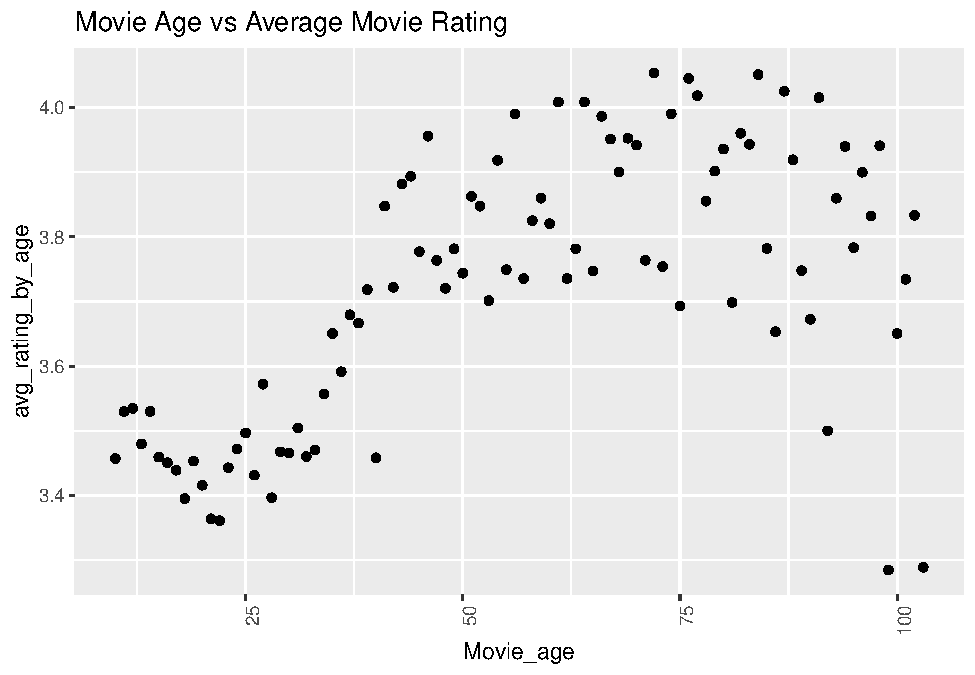
\includegraphics{MovieLensProjectReport_files/figure-latex/MovieAge-1.pdf}
\#Graphical Representation (Point Chart) : Premier Year vs average movie
rating

\begin{Shaded}
\begin{Highlighting}[]
\NormalTok{edx_avg_ratings <-}\StringTok{ }\NormalTok{edx_Movie_Aging_Details }\OperatorTok\StringTok{ }\KeywordTok{group_by}\NormalTok{(Premier_Year) }\OperatorTok\StringTok{ }\KeywordTok{summarise}\NormalTok{(}\DataTypeTok{avg_rating_by_age =} \KeywordTok{mean}\NormalTok{(rating))}
\NormalTok{edx_avg_ratings }\OperatorTok\StringTok{ }\KeywordTok{ggplot}\NormalTok{(}\KeywordTok{aes}\NormalTok{(Premier_Year, avg_rating_by_age)) }\OperatorTok{+}\StringTok{   }\KeywordTok{geom_point}\NormalTok{() }\OperatorTok{+}
\StringTok{  }\KeywordTok{theme}\NormalTok{(}\DataTypeTok{axis.text.x =} \KeywordTok{element_text}\NormalTok{(}\DataTypeTok{angle =} \DecValTok{90}\NormalTok{,}\DataTypeTok{hjust =} \DecValTok{1}\NormalTok{))}\OperatorTok{+}
\StringTok{  }\KeywordTok{ggtitle}\NormalTok{(}\StringTok{"Premier Year vs Average Movie Rating"}\NormalTok{)}
\end{Highlighting}
\end{Shaded}

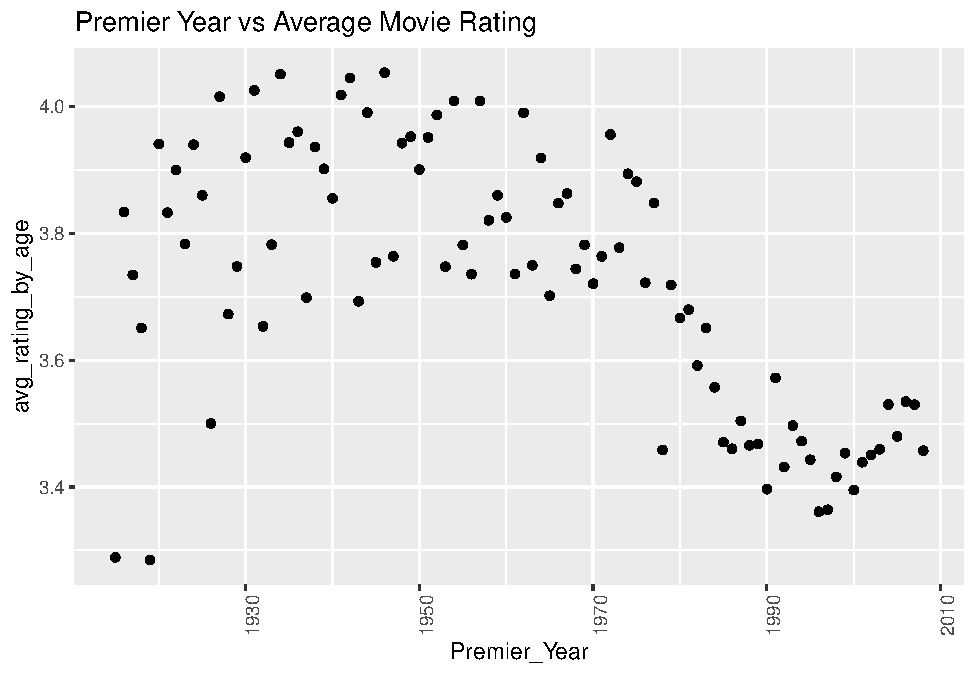
\includegraphics{MovieLensProjectReport_files/figure-latex/Premier_Year-1.pdf}
\#Conclusion: The above two graphical representations of "``Movie Age''
and ``Premier Year'' against Average Movie Rating provide us with the
following two facts: 1. Higher ratings the older a movies is up to 90
years old, then the ratings drop.In other words, Movies from earlier
decades have more volatile ratings which has to be considered during
accuracy calculation. 2. Recent movies get more ratings. Movies earlier
than 1930 get few ratings, whereas newer movies, especially in the 90s
get far more ratings.

\hypertarget{iv.-result}{%
\subsection{IV. Result}\label{iv.-result}}

MovieLens data set is a large data set (size 10M), hence an efficient
method was needed to predict movie ratings. The PENALIZED LEAST SQUARE
approach is based on the mean movie rating. This average is adjusted for
user-effects and movie-effects in order to volatile ratings with respect
to users and movies. To adjust for these effects, a penalty - LAMBDA -
is taken into account.

\#Determine Lambda

\begin{Shaded}
\begin{Highlighting}[]
\CommentTok{#RMSE Calculation}
\NormalTok{RMSE <-}\StringTok{ }\ControlFlowTok{function}\NormalTok{(true_ratings, predicted_ratings)\{}
  \KeywordTok{sqrt}\NormalTok{(}\KeywordTok{mean}\NormalTok{((true_ratings }\OperatorTok{-}\StringTok{ }\NormalTok{predicted_ratings)}\OperatorTok{^}\DecValTok{2}\NormalTok{))}
\NormalTok{\}}
\NormalTok{lambdas <-}\StringTok{ }\KeywordTok{seq}\NormalTok{(}\DecValTok{0}\NormalTok{,}\DecValTok{5}\NormalTok{,.}\DecValTok{5}\NormalTok{)}
\NormalTok{rmses <-}\StringTok{ }\KeywordTok{sapply}\NormalTok{(lambdas, }\ControlFlowTok{function}\NormalTok{(l)\{}
\NormalTok{  mu <-}\StringTok{ }\KeywordTok{mean}\NormalTok{(edx_Movie_Aging_Details}\OperatorTok{$}\NormalTok{rating)}
  
\NormalTok{  b_i <-}\StringTok{ }\NormalTok{edx_Movie_Aging_Details }\OperatorTok
\StringTok{    }\KeywordTok{group_by}\NormalTok{(movieId) }\OperatorTok
\StringTok{    }\KeywordTok{summarize}\NormalTok{(}\DataTypeTok{b_i =} \KeywordTok{sum}\NormalTok{(rating }\OperatorTok{-}\StringTok{ }\NormalTok{mu)}\OperatorTok{/}\NormalTok{(}\KeywordTok{n}\NormalTok{() }\OperatorTok{+}\StringTok{ }\NormalTok{l))}
  
\NormalTok{  b_u <-}\StringTok{ }\NormalTok{edx_Movie_Aging_Details }\OperatorTok
\StringTok{    }\KeywordTok{left_join}\NormalTok{(b_i, }\DataTypeTok{by=}\StringTok{'movieId'}\NormalTok{) }\OperatorTok\StringTok{ }
\StringTok{    }\KeywordTok{group_by}\NormalTok{(userId) }\OperatorTok
\StringTok{    }\KeywordTok{summarize}\NormalTok{(}\DataTypeTok{b_u =} \KeywordTok{sum}\NormalTok{(rating }\OperatorTok{-}\StringTok{ }\NormalTok{b_i }\OperatorTok{-}\StringTok{ }\NormalTok{mu)}\OperatorTok{/}\NormalTok{(}\KeywordTok{n}\NormalTok{() }\OperatorTok{+}\NormalTok{l))}
  
\NormalTok{  predicted_ratings <-}\StringTok{ }\NormalTok{edx_Movie_Aging_Details }\OperatorTok
\StringTok{    }\KeywordTok{left_join}\NormalTok{(b_i, }\DataTypeTok{by =} \StringTok{"movieId"}\NormalTok{) }\OperatorTok
\StringTok{    }\KeywordTok{left_join}\NormalTok{(b_u, }\DataTypeTok{by =} \StringTok{"userId"}\NormalTok{) }\OperatorTok
\StringTok{    }\KeywordTok{mutate}\NormalTok{(}\DataTypeTok{pred =}\NormalTok{ mu }\OperatorTok{+}\StringTok{ }\NormalTok{b_i }\OperatorTok{+}\StringTok{  }\NormalTok{b_u) }\OperatorTok\StringTok{ }\NormalTok{.}\OperatorTok{$}\NormalTok{pred}
  
  \KeywordTok{return}\NormalTok{(}\KeywordTok{RMSE}\NormalTok{(predicted_ratings, edx_Movie_Aging_Details}\OperatorTok{$}\NormalTok{rating))}
\NormalTok{\})}
\CommentTok{#Graphical Representation of Lambda &rmses}
\KeywordTok{qplot}\NormalTok{(lambdas, rmses)}
\end{Highlighting}
\end{Shaded}

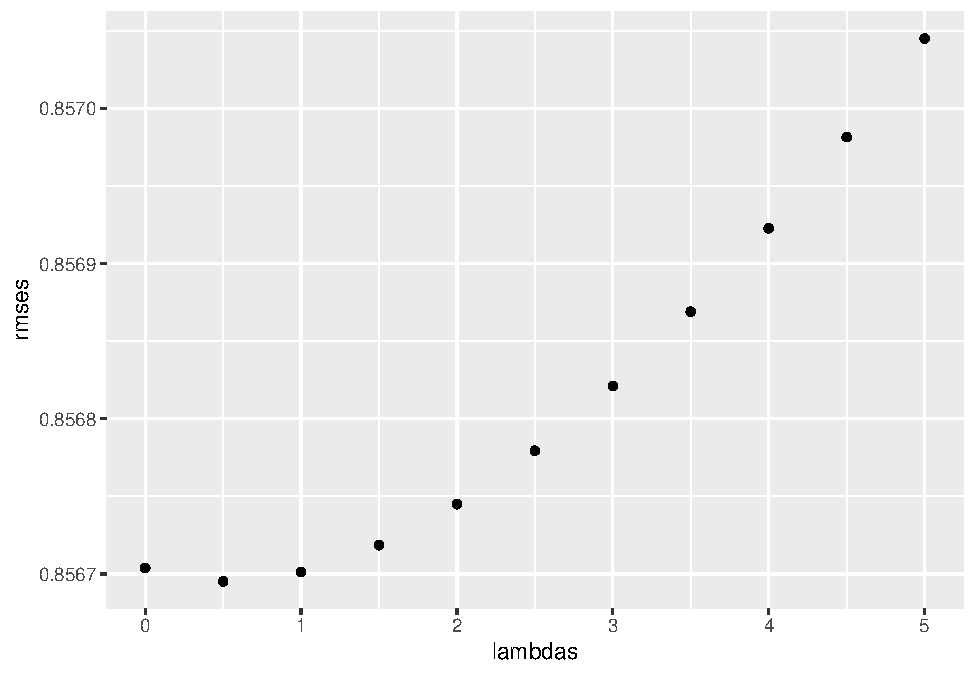
\includegraphics{MovieLensProjectReport_files/figure-latex/RMSE-1.pdf}

\begin{Shaded}
\begin{Highlighting}[]
\NormalTok{lambda <-}\StringTok{ }\NormalTok{lambdas[}\KeywordTok{which.min}\NormalTok{(rmses)]}
\KeywordTok{paste}\NormalTok{(}\StringTok{'Optimal RMSE of'}\NormalTok{,}\KeywordTok{min}\NormalTok{(rmses),}\StringTok{'is achieved with Lambda'}\NormalTok{,lambda)}
\end{Highlighting}
\end{Shaded}

\begin{verbatim}
## [1] "Optimal RMSE of 0.856695227644159 is achieved with Lambda 0.5"
\end{verbatim}

Also, as per the above QPlot, the optimal RMSE is achieved with Lambda =
0.5 \#Predicting the Validation Set using the optimal Lambda = 0.5

\begin{Shaded}
\begin{Highlighting}[]
\NormalTok{mu <-}\StringTok{ }\KeywordTok{mean}\NormalTok{(validation}\OperatorTok{$}\NormalTok{rating)}
\NormalTok{l <-}\StringTok{ }\NormalTok{lambda}
\NormalTok{b_i <-}\StringTok{ }\NormalTok{validation }\OperatorTok
\StringTok{  }\KeywordTok{group_by}\NormalTok{(movieId) }\OperatorTok
\StringTok{  }\KeywordTok{summarize}\NormalTok{(}\DataTypeTok{b_i =} \KeywordTok{sum}\NormalTok{(rating }\OperatorTok{-}\StringTok{ }\NormalTok{mu)}\OperatorTok{/}\NormalTok{(}\KeywordTok{n}\NormalTok{() }\OperatorTok{+}\StringTok{ }\NormalTok{l))}

\NormalTok{b_u <-}\StringTok{ }\NormalTok{validation }\OperatorTok
\StringTok{  }\KeywordTok{left_join}\NormalTok{(b_i, }\DataTypeTok{by=}\StringTok{'movieId'}\NormalTok{) }\OperatorTok\StringTok{ }
\StringTok{  }\KeywordTok{group_by}\NormalTok{(userId) }\OperatorTok
\StringTok{  }\KeywordTok{summarize}\NormalTok{(}\DataTypeTok{b_u =} \KeywordTok{sum}\NormalTok{(rating }\OperatorTok{-}\StringTok{ }\NormalTok{b_i }\OperatorTok{-}\StringTok{ }\NormalTok{mu)}\OperatorTok{/}\NormalTok{(}\KeywordTok{n}\NormalTok{() }\OperatorTok{+}\NormalTok{l))}

\NormalTok{predicted_ratings <-}\StringTok{ }\NormalTok{validation }\OperatorTok
\StringTok{  }\KeywordTok{left_join}\NormalTok{(b_i, }\DataTypeTok{by =} \StringTok{"movieId"}\NormalTok{) }\OperatorTok
\StringTok{  }\KeywordTok{left_join}\NormalTok{(b_u, }\DataTypeTok{by =} \StringTok{"userId"}\NormalTok{) }\OperatorTok
\StringTok{  }\KeywordTok{mutate}\NormalTok{(}\DataTypeTok{pred =}\NormalTok{ mu }\OperatorTok{+}\StringTok{ }\NormalTok{b_i }\OperatorTok{+}\StringTok{  }\NormalTok{b_u) }\OperatorTok\StringTok{ }\NormalTok{.}\OperatorTok{$}\NormalTok{pred}

\KeywordTok{RMSE}\NormalTok{(predicted_ratings, validation}\OperatorTok{$}\NormalTok{rating)}
\end{Highlighting}
\end{Shaded}

\begin{verbatim}
## [1] 0.8258487
\end{verbatim}

After exploring the movies through graphical representations and
calculating RMSE, it can be concluded that the best predictor for
ratings was movieId, userId. The age of the movie didn't change the RMSE
The RMSE calculated and validated against the Validation set - 0.8258487

\end{document}
